\scanpage{105}
\mspage{104}%
by a \rlap{right}left $H'$-torsor $Q$.

Subject to the verification left pending just now, one then finds that the datum of a``\uline{filtered} fiber functor''$F$ on $\underline{C}$ over $k$ amounts to the datum

(i) of a fibre functor $F'$ \deleted{graded of type} (whence a Galois group\deleted{d} $G'=\underline{\operatorname{Aut}}(F')$ );\rlap{\tikz[baseline=0pt,x=1em,y=1em]{\draw (0,-.5)--(.03,-.65);}}

(ii) Of a grad\rlap{d}ing of type $\underline{Z}$ of $F'$, i.e. a homomorphism
\[
i_1:\underline{G}_m\handwritten{\longrightarrow}G',
\]
\margin{\tikz[baseline=0pt,x=1em,y=1em]{\draw (0,0)--(.12,.2)--(.08,.3);}}which allows one to define as above a subgroup $H'_{i_1}$ of $G'$ ;

(iii) Of a \rlap{right}left torsor $Q'$ under $H'_{i_1}$.

To these data, one simply associates the twisted fiber functor
\[
F=F'\mathop{\handwritten{\wedge}}\limits^{H'_{i_1}}Q',
\]
$F$ being filtered by the filtration deduced from that of $F'$ \deleted{(\unsure{via} the \unsure{gradin|grading}} (associated to the grading of $F'$) by twisting by $Q'$.

\deleted{NB In the case where $F$ is the De Rham functor on the category of motives over $k$, one proves (using the general yoga of motives - it is possible that one uses the Hodge conjectures for this ...) that the group $H'$ is an inverse limit of \deleted{\inserted{smooth}} \inserted{unipotent} algebraic groups \deleted{with \uline{solvable} connected components\unsure{.} Thus} \unsure{$\mathbb{S}$|S}upposing one restricts oneself to a \deleted{of} finitely generated category of motives, and supposing $G$ is connected, one also finds that $H'$ is connected, hence being solvable, one finds}

One easily sees that the group $H'$ is necessarily an inverse limit of \uline{unipotent} algebraic groups. One immediately concludes from this that if $\underline{C}$ is finitely generated (or, more generally, countably \inserted{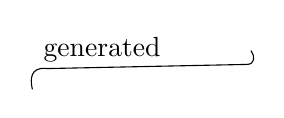
\begin{tikzpicture}[baseline=-.2ex,x=1em,y=1em]
\node[anchor=base west] at (0,.5) {\handwritten{\unsure{generated}}};
\draw (-.05,-.7) .. controls (-.2,-.05) and (.1,.1) .. (.5,.05) -- (7.7,.2) .. controls (8,.2) and (8,.5) .. (7.85,.7);
\end{tikzpicture}}, so that $G'$ \deleted{is} hence also $H'$ is an inverse limit of a \uline{sequence} of algebraic groups)\margin{\tikz[baseline=0pt,x=1em,y=1em]{\draw (0,0)--(.16,.2);}} then every torsor under $H'$ is trivial; this means here that every filtered fibre functor is in fact associated to a graded fibre functor (by taking the filtration corresponding to the grading)
